% !TEX TS-program = XeLaTeX
% use the following command:
% all document files must be coded in UTF-8
\documentclass[english]{textolivre}
% build HTML with: make4ht -e build.lua -c textolivre.cfg -x -u article "fn-in,svg,pic-align"

\journalname{Texto Livre}
\thevolume{19}
%\thenumber{1} % old template
\theyear{2026}
\receiveddate{\DTMdisplaydate{2025}{12}{6}{-1}} % YYYY MM DD
\accepteddate{\DTMdisplaydate{2026}{2}{13}{-1}}
\publisheddate{\DTMdisplaydate{2026}{8}{10}{-1}}
\corrauthor{Amjad Mohammad Badah}
\articledoi{10.1590/1983-3652.2026.63334}
%\articleid{NNNN} % if the article ID is not the last 5 numbers of its DOI, provide it using \articleid{} commmand 
% list of available sesscions in the journal: articles, dossier, reports, essays, reviews, interviews, editorial
\articlesessionname{articles}
\runningauthor{Badah and Esteban-Segura} 
%\editorname{Leonardo Araújo} % old template
\sectioneditorname{Nome e sobrenome~\orcid{0000-0003-1861-3609}}
\layouteditorname{Nome e sobrenome~\orcid{0000-0003-3884-2177}}

\title{Translation in the Age of AI: Insights from Palestinian Professional Translators}
\othertitle{Tradução na era da IA: perspectivas de tradutores profissionais palestinos}
% if there is a third language title, add here:
%\othertitle{Artikelvorlage zur Einreichung beim Texto Livre Journal}

\author[1]{Amjad Mohammad Badah~\orcid{0000-0003-2729-1875}\thanks{Email: \href{mailto:amjad.badah@uma.es}{amjad.badah@uma.es}}}
\author[2]{Laura Esteban-Segura~\orcid{0000-0001-7721-2210}\thanks{Email: \href{mailto:lesteban@uma.es}{lesteban@uma.es}}}
\affil[1]{University of Málaga, Doctoral Programme in Linguistics, Literature and Translation, Málaga, Spain.}
\affil[2]{University of Málaga, Research Institute of Multilingual Language Technologies, Málaga, Spain.}

\addbibresource{article.bib}
% use biber instead of bibtex
% $ biber article

% used to create dummy text for the template file
\definecolor{dark-gray}{gray}{0.35} % color used to display dummy texts
\usepackage{lipsum}
\SetLipsumParListSurrounders{\colorlet{oldcolor}{.}\color{dark-gray}}{\color{oldcolor}}

% used here only to provide the XeLaTeX and BibTeX logos
\usepackage{hologo}

% if you use multirows in a table, include the multirow package
\usepackage{multirow}

% provides sidewaysfigure environment
\usepackage{rotating}

% CUSTOM EPIGRAPH - BEGIN 
%%% https://tex.stackexchange.com/questions/193178/specific-epigraph-style
\usepackage{epigraph}
\renewcommand\textflush{flushright}
\makeatletter
\newlength\epitextskip
\pretocmd{\@epitext}{\em}{}{}
\apptocmd{\@epitext}{\em}{}{}
\patchcmd{\epigraph}{\@epitext{#1}\\}{\@epitext{#1}\\[\epitextskip]}{}{}
\makeatother
\setlength\epigraphrule{0pt}
\setlength\epitextskip{0.5ex}
\setlength\epigraphwidth{.7\textwidth}
% CUSTOM EPIGRAPH - END

% to use IPA symbols in unicode add
%\usepackage{fontspec}
%\newfontfamily\ipafont{CMU Serif}
%\newcommand{\ipa}[1]{{\ipafont #1}}
% and in the text you may use the \ipa{...} command passing the symbols in unicode

% LANGUAGE - BEGIN
% ARABIC
% for languages that use special fonts, you must provide the typeface that will be used
% \setotherlanguage{arabic}
% \newfontfamily\arabicfont[Script=Arabic]{Amiri}
% \newfontfamily\arabicfontsf[Script=Arabic]{Amiri}
% \newfontfamily\arabicfonttt[Script=Arabic]{Amiri}
%
% in the article, to add arabic text use: \textlang{arabic}{ ... }
%
% RUSSIAN
% for russian text we also need to define fonts with support for Cyrillic script
% \usepackage{fontspec}
% \setotherlanguage{russian}
% \newfontfamily\cyrillicfont{Times New Roman}
% \newfontfamily\cyrillicfontsf{Times New Roman}[Script=Cyrillic]
% \newfontfamily\cyrillicfonttt{Times New Roman}[Script=Cyrillic]
%
% in the text use \begin{russian} ... \end{russian}
% LANGUAGE - END

% EMOJIS - BEGIN
% to use emoticons in your manuscript
% https://stackoverflow.com/questions/190145/how-to-insert-emoticons-in-latex/57076064
% using font Symbola, which has full support
% the font may be downloaded at:
% https://dn-works.com/ufas/
% add to preamble:
% \newfontfamily\Symbola{Symbola}
% in the text use:
% {\Symbola }
% EMOJIS - END

% LABEL REFERENCE TO DESCRIPTIVE LIST - BEGIN
% reference itens in a descriptive list using their labels instead of numbers
% insert the code below in the preambule:
%\makeatletter
%\let\orgdescriptionlabel\descriptionlabel
%\renewcommand*{\descriptionlabel}[1]{%
%  \let\orglabel\label
%  \let\label\@gobble
%  \phantomsection
%  \edef\@currentlabel{#1\unskip}%
%  \let\label\orglabel
%  \orgdescriptionlabel{#1}%
%}
%\makeatother
%
% in your document, use as illustraded here:
%\begin{description}
%  \item[first\label{itm1}] this is only an example;
%  % ...  add more items
%\end{description}
% LABEL REFERENCE TO DESCRIPTIVE LIST - END


% add line numbers for submission
%\usepackage{lineno}
%\linenumbers

\begin{document}
\maketitle

\begin{polyabstract}
\begin{abstract}
With the increasing integration of Artificial Intelligence (AI) in many fields, including translation, understanding how professional translators adopt and experience these tools has become a pressing need, particularly in under-researched contexts such as Palestine. This study examines the use of AI-powered machine translation tools by Palestinian professional translators in their translation tasks. It mainly addresses the extent to which Palestinian translators use AI-powered translation tools and how they perceive these tools in terms of their advantages, challenges, cultural meaning, and ethical considerations. Using a mixed-methods approach, data were collected through a questionnaire distributed to translators and in-depth interviews conducted with experienced practitioners. The questionnaire gathered 86 responses from professional translators working in Palestine. The interviews were conducted with seven professional translators who were purposefully selected based on their level of experience and the nature of their work. The results revealed that AI-powered machine translation tools are widely used among translators, with 83.7\% of respondents reporting regular use. The findings also revealed that while these tools enhance speed and efficiency, translators exercise cautious trust and emphasize human revision to maintain linguistic accuracy, cultural relevance, and ethical standards. This study contributes to Translation Studies by providing empirical evidence on AI adoption in professional practice, highlighting practical implications for translator training and workflow integration of AI tools, and informing future research on the evolving role of AI in the translation industry.

\keywords{AI-powered Machine Translation \sep Translation Industry \sep Professional Translators \sep Google Translate \sep ChatGPT}
\end{abstract}

\begin{portuguese}
\begin{abstract}
Com a crescente integração da Inteligência Artificial (IA) em diversas áreas, incluindo a tradução, compreender como os tradutores profissionais adotam e vivenciam essas ferramentas tornou-se uma necessidade premente, especialmente em contextos pouco pesquisados como a Palestina. Este estudo examina o uso de ferramentas de tradução automática baseadas em IA por tradutores profissionais palestinos em suas tarefas de tradução. Aborda-se principalmente a extensão do uso de ferramentas de tradução baseadas em IA por tradutores palestinos e a forma como percebem essas ferramentas em termos de vantagens, desafios, significado cultural e considerações éticas. Utilizando uma abordagem de métodos mistos, os dados foram coletados por meio de um questionário distribuído a tradutores e entrevistas em profundidade realizadas com profissionais experientes. O questionário obteve 86 respostas de tradutores profissionais que atuam na Palestina. As entrevistas foram conduzidas com sete tradutores profissionais selecionados intencionalmente com base em seu nível de experiência e na natureza de seu trabalho. Os resultados revelaram que as ferramentas de tradução automática baseadas em IA são amplamente utilizadas entre os tradutores, com 83,7\% dos respondentes relatando uso regular. Os resultados também revelaram que, embora essas ferramentas aumentem a velocidade e a eficiência, os tradutores demonstram cautela ao confiar nelas e enfatizam a revisão humana para manter a precisão linguística, a relevância cultural e os padrões éticos. Este estudo contribui para os Estudos da Tradução ao fornecer evidências empíricas sobre a adoção da IA na prática profissional, destacando as implicações práticas para o treinamento de tradutores e a integração de ferramentas de IA no fluxo de trabalho, bem como orientando pesquisas futuras sobre o papel em evolução da IA no setor de tradução.

\keywords{Tradução automática com IA \sep Setor de tradução \sep Tradutores profissionais \sep Google Tradutor \sep ChatGPT}
\end{abstract}
\end{portuguese}
% if there is another abstract, insert it here using the same scheme
\end{polyabstract}

\section{Introduction}\label{sec-intro}
The landscape of Translation Studies has undergone significant changes over the past few years. One of the key advancements in this field is the introduction of Artificial Intelligence (AI) in the translation industry. In Palestine, as in many other countries, professional translators are beginning to integrate AI-powered tools into their translation tasks. Professional translators are increasingly relying on AI-powered tools in their daily workflows \cite{OmarSalih2024Postediting}, raising important questions about the role of these technologies in shaping the modern translation industry. However, while these tools offer significant efficiency advances, their autonomous use remains limited, as translators still need to intervene to address issues of accuracy, tone, and naturalness. Human expertise is expected to play a significant role in ensuring high-quality translation \cite{AlKaabiEtAl2024CulturalConnotations,Shahmerdanova2025AITranslation}.

One of the key advantages of using AI in professional translation settings is the improvement of productivity and efficiency \cite{ShormaniAlSohbani2025TranslationIndustry}. AI-powered tools enable translators to produce faster drafts and manage large volumes of content with greater speed. Such tools can assist in maintaining consistency in terminology and style, particularly in large-scale projects, reducing human errors and thus ensuring the output quality. Within the Palestinian translation sector, these developments are attracting growing attention as translators navigate the balance between AI-assisted efficiency and the preservation of human expertise. In this context, translators are becoming more concerned about being replaced by AI-powered tools due to such benefits \cite{KirovMalamin2022TranslatorsAI,MoneusSahari2024LegalTranslation}. This spreading interest is further increased by the rapid developments in the AI field that have narrowed the gap between human and machine output.

On the other hand, the use of AI in translation is still encountering some limitations that hinder its complete effectiveness in the translation industry. Among these limitations is the lack of cultural understanding of both the target and source texts and cultures. This insufficiency may lead to inaccurate or inappropriate translations \cite{Shahmerdanova2025AITranslation}. Most importantly, the use of AI in translation raises ethical concerns related to data privacy, intellectual property rights, and accountability. Regarding accountability, for instance, it is difficult to assign responsibility when the target text is generated by an AI-powered tool. The potential errors or misinterpretations cannot be attributed to non-humans. However, if the text is transferred by a human translator, then that individual can be held legally and ethically accountable for the quality and accuracy of the output.

Given the current relevance of the topic, research on AI use in translation by professional translators has gained momentum in the literature, yet specific aspects remain underexplored, particularly within the Palestinian context. Additionally, the studies that have addressed the fields of AI and translation focused on the effectiveness and the technical performance of AI-powered tools on the translation product. This study aims to explore the usage of AI among professional translators in Palestine and their attitudes toward it in terms of its advantages, limitations, cultural understanding, and ethical considerations. This paper examines how Palestinian professional translators are engaging with AI-powered tools in practice. Filling this gap is significant to capture the reality of translation work in Palestine and to inform local translation training programs, academic majors, and professional practice.

The study then tries to answer the following two major questions: (1) To what extent do Palestinian translators use AI-powered translation tools, and what are their usage patterns and satisfaction levels with these tools?; and (2) How do professional translators perceive the use of AI-powered translation tools in their work, particularly regarding potential advantages and challenges, cultural meaning, and ethical considerations?

By investigating these two questions, the current study aims to provide insights into how translators are integrating AI tools into their translation tasks and how they evaluate the efficiency and quality of these tools. It also explores how the translators address emerging ethical and cultural concerns in professional contexts. Arguably, the study’s novelty lies in its use of a mixed-methods approach to investigate the adoption and professional experiences of AI-powered translation tools among Palestinian translators, making it the first study of its kind in the Palestinian context and addressing both practical and ethical dimensions rarely examined in prior research.

\section{Literature Review}\label{sec-normas}
AI has increasingly influenced the translation landscape during the last few years, particularly with the rise of free AI-powered machine translation tools \cite{OmarSalih2024Postediting}. The emergence of AI has greatly revolutionized this industry \cite{MohamedEtAl2024AITranslationReview}. This review examines key themes and concepts related to the application of AI in the translation process, beginning with an overview of AI’s role in reshaping the translation industry landscape. In this section, both the main advantages and challenges associated with AI employment in the translation process are also highlighted. Moreover, it addresses the technology adoption by professional translators. Finally, it ends by referring to similar studies that were conducted in similar contexts.

\subsection{Overview of AI-Powered Translation}\label{sec-conduta}
The application of AI-powered technologies to translation has become an important topic of interest for all stakeholders, including researchers, academics, professional practitioners, and clients. Given that AI continues to evolve remarkably in the translation field, it raises important questions about human involvement in an increasingly automated landscape. While the history of AI in translation, from Statistical Machine Translation (SMT) to Neural Machine Translation (NMT), is well documented, understanding this evolution is important for contextualizing current professional practices and the adoption of AI tools among translators. Taking into account \posscite{MohamedEtAl2024AITranslationReview} AI-powered translation approaches, it could be argued that AI-powered technologies have evolved rapidly (see \Cref{fig1}) from statistical-based machine systems to more advanced methods like reinforcement learning, becoming integral to both professional and everyday translation contexts. It is worth mentioning that some items, however, represent a training method, such as reinforcement learning, or a testing scenario, like Zero-Shot Translation, rather than a translation paradigm.

\begin{figure}[htbp]
\centering
\begin{minipage}{.7\textwidth}
 
\includegraphics[width=\textwidth]{Fig1.png}
 \caption{AI-Based Translation Approaches.}
 \label{fig1}
 \source{\textcite[p. 25555]{MohamedEtAl2024AITranslationReview}.}
\end{minipage}
\end{figure}

The current research highlights the important technological advancements in AI-powered translation, from NMT to Large Language Models (LLMs) represented by chatbots like ChatGPT, DeepSeek, Copilot, etc. The key developments include the implementation of sequence-to-sequence and transformer models that have substantially enhanced translation accuracy \cite{Siu2024TranslationAI}. Such advancement has not only influenced the quality of the translation output but also played a crucial role in issues such as speed and cost-effectiveness. In addition, AI-powered machine translation has contributed to greater consistency and naturalness across a large volume of texts. Nevertheless, it could be argued that improvements in fluency do not always correspond to deeper semantic or pragmatic accuracy, especially in culturally sensitive contexts. This trend has created new dynamics in the professional translation market, where human translators are increasingly expected to combine their expertise with AI-assisted tools to provide higher-quality translations that consider different types of real-world contexts.


\subsection{Advantages of Using AI-Powered Tools in Translation}\label{sec-fmt-manuscrito}
AI-powered translation technologies have significantly increased accessibility to translation services and revolutionized the translation industry during the last few years. They offer many advantages, such as speed, cost-effectiveness, and improved consistency in handling text irrespective of its type. These tools offer significant benefits, including improved translation accuracy and multilingual communication \cite{HuangLiCheung2025LinguisticComplexity,Shahmerdanova2025AITranslation,VieiraOHaganOSullivan2021SocietalImpacts}. \textcite{MohamedEtAl2024AITranslationReview} argue that the rise of AI in the translation industry has introduced new opportunities that could bridge communication gaps and enhance cross-cultural understanding. However, opinions in the literature are mixed, with some studies portraying AI as a transformative tool, while others caution that its benefits may be context-dependent and not uniformly realized across all translation tasks.

With the latest advancement in LLMs, these tools now generate immediate high-quality translations without the extensive training times typical of older machine translation systems. Importantly, AI can also help translators and even normal users by automating low-value tasks and thus letting them focus on post-editing and quality assurance. Human expertise, however, remains essential for conveying emotions and cultural references that AI cannot fully capture.

\subsection{Challenges of AI-Powered Machine Translation}\label{sec-formato}
Even though there are many advantages of using AI tools in the translation profession, several of such tools face challenges that influence translation effectiveness, accuracy, and reliability. Key issues include understanding the real-world context and grasping cultural elements and idiomatic expressions. AI translation challenges lie in the translation of idiomatic expressions, addressing cultural sensitivity, and maintaining emotional equivalence in translations \cite{AlsharifEtAl2026MetaphorChatGPT,BadahEtAl2025LegalTranslationAI,Shahmerdanova2025AITranslation}. Indeed, idiomatic and cultural expressions are considered a difficult area for AI translation systems as they are often unique to a particular language or region and cannot be translated literally. In this vein, \textcite{AlyamiAlzubi2025HumanTranslatorsAI,AlsharifEtAl2026MetaphorChatGPT} state that AI translation struggles with literary and cultural translations because of figurative language and cultural references. While there is broad agreement on these limitations, scholars differ regarding whether ongoing advances in LLMs substantially mitigate these weaknesses.

The rapid incorporation of AI into language learning environments is transforming translation pedagogy while introducing significant ethical and behavioral concerns \cite{ZhangLi2026EthicalPerceptions}. While ethical considerations are mentioned in the translation context, specific text types that are considered to be sensitive, such as legal and medical documents, raise additional ethical concerns and accuracy requirements \cite{Shahmerdanova2025AITranslation,vanKolfschootenEtAl2025HealthcareAI}. AI-powered translation may fail to meet such precision and accountability standards. Besides, there is a potential risk that sensitive or confidential information included in those documents could be exposed to others. Another important issue is related to the bias caused by AI translation systems. In this vein, \textcite{ZhangLi2026EthicalPerceptions} note that algorithmic bias and inequitable outputs have long been central concerns in language technology research, particularly within translation contexts. AI-powered translation tools are trained on specific datasets by developers, who have their own views and biases and may include prejudiced content. \textcite{TomalinEtAl2021BiasReduction} claim that NMT systems are known to exhibit gender bias due to patterns present in their training datasets. This creates systemic shortcomings that affect other language users. Another key challenge for AI translation technologies lies in handling the complex structure of some languages, such as Arabic. The richness of morphology and context-dependent meanings often hinder accurate and reliable translation. In this vein, \textcite{Bousetouane2024ArabicTranslationAI} argues that Arabic translation is particularly challenging due to its rich morphology and complex syntax. These language-specific challenges suggest that AI performance is uneven across linguistic contexts, a point that has not been sufficiently explored in many large-scale studies.

In light of all these challenges, the human touch is always needed to ensure complete contextual understanding, safeguard content privacy, and avoid potential biases. Human translators have critical judgment that AI tools cannot fully imitate. \textcite{Shahmerdanova2025AITranslation} states that experts recommend a hybrid translation mode that integrates AI’s technological strengths with human expertise to address AI limitations while maintaining cultural and linguistic integrity. This hybrid perspective has gained increasing support in recent literature, although empirical evidence from real professional settings remains relatively limited due to the recent emergence of AI-powered translation tools.


\subsection{Professional Translators and Technology Adoption}\label{sec-modelo}
In this study, a professional translator is operationally defined as an individual actively engaged in paid translation work. Consistent with prior research emphasizing both professional engagement and experience, participants are further categorized according to their years of translation practice (1–5 years, 6–10 years, 11–15 years, and more than 16 years) and employment type (full-time, part-time, or freelance). This operationalization allows the study to capture varying levels of professional expertise while emphasizing both practical experience and professional engagement.

Professional translators have remarkably integrated technology into their work in an attempt to enhance the efficiency and quality of the translation outcome and meet growing market demands and tight deadlines. Such adoption has started with the use of Computer-Assisted Translation (CAT) tools, and later machine translation. NMT has emerged as the dominant paradigm in the machine translation community \cite{WangEtAl2022ProgressMT}. However, the pace and depth of adoption appear to vary considerably across professional contexts and experience levels.

With the emergence of new translation technologies, including NMT and LLMs, translators are now increasingly employing these technologies for their numerous advantages, particularly in terms of speed and accuracy. This has affected the translator’s roles, particularly in handling minor tasks. \textcite{AlyamiAlzubi2025HumanTranslatorsAI} found that AI has shifted translators’ roles toward editing and post-editing the content generated by AI. However, the degree of technology adoption among professional translators is influenced by many factors, including experience level, urgency, and text types. Such adoption, on the other hand, depends on the translators’ ability to balance technical proficiency with linguistic competency. This indicates that adoption is not merely a technical issue but also a professional and cognitive adjustment process.

Many translators share concerns that AI translation technologies may replace them. \textcite{KirovMalamin2022TranslatorsAI} found that translators consider AI and automation real threats to the profession of translation. Nevertheless, such a perspective is open to debate, as translators should consider technology a supportive tool that enhances productivity and quality rather than fully replacing their human expertise. Indeed, the literature shows a clear divide between optimistic views that strongly support AI adoption and more cautious perspectives that highlight its limitations. The latter may include the use of post-editing techniques to refine machine-generated translations and ensure linguistic accuracy and cultural appropriateness. In this context, translators are increasingly expected to develop digital literacy and AI-assisted translation skills. Ultimately, the human translator’s critical thinking, creativity, and contextual understanding remain irreplaceable elements of high-quality translation. By integrating AI technology with human expertise, the future of translation can balance efficiency with cultural and linguistic integrity and further foster global communication \cite{Shahmerdanova2025AITranslation}.

\subsection{Similar Studies}\label{sec-organizacao}
Many recent translation-focused studies have investigated the extent to which professional translators use AI-powered translation tools and how they perceive these technologies in their work. \textcite{MoneusSahari2024LegalTranslation} state that the rapid development of AI has sparked increasing debate about its potential impact on human existence, with perspectives ranging from viewing AI as a tool that supports human development to concerns that it may create multiple challenges in the future. \textcite{AlyamiAlzubi2025HumanTranslatorsAI} surveyed the perceptions of professional translators, translation students, and instructors on the evolving role of human translators in the age of AI. The study indicated that while AI translation systems have improved productivity and consistency, significant challenges remain in literary and cultural translation due to figurative language and cultural references. Ethical concerns such as data privacy and the risk of deskilling were also prominent. The translators emphasized the need for ongoing skill development and AI literacy to balance automation with human expertise. These findings broadly align with the growing consensus that AI enhances workflow efficiency while still requiring substantial human intervention. \posscite{JimenezCrespo2024HumanCentredAI} survey of 41 professional translators examined attitudes toward control and autonomy in the use of AI and translation technologies. The results showed that a majority of translators reported high levels of perceived control and autonomy over their current technology. However, the adoption of generative AI tools remains relatively low. This contrasts with studies reporting widespread general AI use, suggesting that adoption patterns may depend on tool type and professional context. Another relevant survey, conducted by \textcite{KirovMalamin2022TranslatorsAI}, focused on Bulgarian professional translators and their attitudes toward AI and automation. The results demonstrated that most translators perceive AI as a tool that relieves them of routine and technical tasks. It allows them to focus more on post-editing and higher-level linguistic work. Translators reported that their roles are evolving with increased emphasis on editing machine-generated texts and training AI systems.

Based on the overview above, it is clear that while recent studies have highlighted the widespread use of AI-powered translation tools among professional translators and examined their perceived benefits and challenges, there remains a significant gap in the literature. Most existing studies either focus on experimental comparisons between human and AI translation or explore only isolated aspects of professional practice, often neglecting the integration of AI tools into day-to-day translation workflows. There is also limited research that combines large-scale survey data with in-depth qualitative insights from experienced practitioners, particularly in under-researched contexts such as Palestine. Addressing this gap is critical for moving beyond perception-based studies toward evidence grounded in actual professional practice. This study is novel in its mixed-methods approach, integrating quantitative and qualitative data to provide a comprehensive understanding of how Palestinian professional translators adopt, use, and evaluate AI-powered translation tools in practice. By exploring practical experiences, satisfaction levels, challenges, cultural considerations, and ethical implications, the study offers methodological and contextual innovation and contributes new empirical evidence to Translation Studies.

\section{Methodology}\label{sec-organizacao-latex}

\subsection{Research Design}\label{sec-titulo}
This study adopted a mixed-method research design to investigate the perceptions, experiences, and practices of professional translators. The researchers primarily employed a survey method through a structured questionnaire to gather quantitative data. The questionnaire was designed specifically for professional translators. To enhance the validity of the questionnaire, it was developed based on existing literature, prior studies on AI in translation, and the authors’ professional expertise to ensure alignment with the research objectives. Content validity was further strengthened through three expert reviewers, where the clarity, relevance, and comprehensiveness of each item were assessed, and their feedback was used to refine the questions. The questionnaire was developed using Google Forms, which allowed for easy distribution and efficient data collection. It consists of closed-ended questions to provide standardized data that can be statistically analyzed to identify dominant trends and patterns. To ensure reliability, a pilot test was conducted with a small group of translators to check for clarity, consistency, and understanding of the questions. Any ambiguous items were revised. The standardized administration and clearly structured questions further strengthened the instrument’s reliability.

For the qualitative part of the study, structured interviews were conducted with seven professional translators. The seven interviewees were purposefully selected using a maximum-variation sampling strategy to ensure representation across different professional profiles within the Palestinian translation community. Selection criteria included active engagement in paid translation work and diversity of professional roles (e.g., translation instructors, academic translators, licensed practitioners, and postgraduate students working in the field of translation). Participants’ years of professional experience were also considered to reflect variation across career stages. This purposive sampling ensured that the participants were not treated as a homogeneous group, allowing the study to capture diverse perspectives, practices, and attitudes toward AI-assisted translation. It is worth mentioning that initial recruitment was facilitated through the researchers’ professional networks within the Palestinian translation community. However, all participants’ eligibility and professional status were systematically confirmed through self-reported background information collected during the interviews.

The interviews aimed to collect detailed and structured information to systematically identify patterns and trends in participants’ professional practices using AI-powered translation tools, their perceptions of the advantages and challenges of AI integration, and their perspectives on the ethical issues associated with AI in professional translation. Each interview lasted nearly 20 to 30 minutes and was designed to complement the questionnaire data by providing rich, context-specific information that could not be obtained through survey responses alone.

\subsection{Data Collection}\label{sec-autores}
Data collection was conducted using a structured questionnaire for quantitative data and structured interviews for qualitative insights. The questionnaire was distributed electronically to professional translators and included closed-ended items to measure adoption rates of AI, usage patterns, and satisfaction levels. Interview data were collected from purposefully selected participants to ensure diversity in professional roles and experience. All collected data were systematically classified. The quantitative responses were organized into categories corresponding to research questions and analyzed using descriptive statistics, while qualitative responses were transcribed, coded, and grouped thematically to identify recurring patterns, perceptions, and challenges in AI-assisted translation practice.

\subsection{Study Population}\label{sec-idioma}
The study population consisted of Palestinian professional translators who use AI tools in their translation work. The questionnaire was distributed to a large number of translators through professional groups on social media platforms to ensure broad participation. A total of 86 translators responded to the questionnaire, of whom 21\% were male and 79\% were female. Their educational backgrounds varied, with 45\% holding a bachelor’s degree, 36\% a master’s degree, and 16\% a PhD. Regarding the interviews, the participants were purposefully selected based on their level of translation experience to ensure the collection of insightful and experience-based information relevant to the study objectives. In terms of professional experience, 58.10\% of the participants have 1–5 years of translation experience, 12.80\% have 6–10 years, 14\% have 11–15 years, and 15.10\% have more than 16 years of professional experience. In line with the study’s operational definition, all participants were actively engaged in paid translation work and were therefore considered professional translators, although they represent different career stages within the profession. Regarding the nature of their work, the majority of participants (79.1\%) were freelance translators.

\subsection{Data Analysis}\label{sec-resumo}
The collected data were analyzed using both quantitative and qualitative analytical approaches consistent with the mixed-method design of the study. Quantitative data obtained from the questionnaire were analyzed using descriptive statistics, including frequencies and percentages, to identify patterns. The results were presented in figures for clarity. For the qualitative data, the interview responses were transcribed and thematically analyzed to uncover recurring ideas and themes related to AI integration in translation practice. Thematic analysis involved reading the transcripts multiple times, coding key segments, and grouping similar codes into overarching themes. Such a combination of statistical and thematic analyses allowed for a comprehensive understanding of translators’ attitudes and practices through integrating numerical findings with rich narrative insights. Regarding data reporting, the results were described in a structured and systematic manner aligned with the research questions. Quantitative findings from the questionnaire were presented using figures and descriptive statistics to clearly illustrate the rates. Qualitative findings from the interviews were organized thematically, with key quotes included to support the interpretation of each theme.

\section{Results}\label{sec-secoes}
This section outlines the results of both the quantitative and qualitative data obtained from the study instruments. The qualitative data are presented in figures with a brief description of the emerging patterns and trends. On the other hand, the qualitative data are organized thematically with a brief description of each theme supported by selected quotations from the participants.

\subsection{RQ 1: To what extent do Palestinian translators use AI-powered translation tools, and what are their usage patterns and satisfaction levels with these tools?}\label{sec-format-simple}
This subsection addresses the first research question by analyzing the data collected through the first research instrument, namely, the questionnaire. It examines the extent to which Palestinian translators use AI-powered translation tools, as well as their usage patterns and levels of satisfaction with these technologies.

\begin{enumerate}
    \item \textbf{AI Adoption in Translation}

    The results showed that the majority of participants (83.7\%) reported using AI-powered translation tools in their work, as shown in \Cref{fig2}. This high adoption rate suggests that AI technologies have become an integral component of contemporary translation workflows among Palestinian translators. It also reflects the increasing reliance on digital tools to enhance efficiency in professional translation practice.

\begin{figure}[htbp]
\centering
\begin{minipage}{.8\textwidth}
 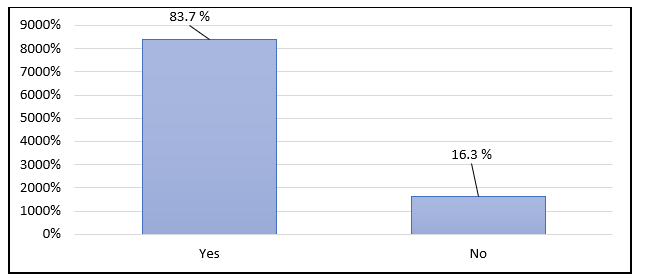
\includegraphics[width=\textwidth]{Figure 2.png}
 \caption{Usage of AI-Powered Tools among Translators.}
 \label{fig2}
 \source{The authors.}
\end{minipage}
\end{figure}

\item \textbf{Translation Tools Used}

The survey results indicate that Google Translate emerges as the dominant platform used by the majority of translators, as depicted in \Cref{fig3}. ChatGPT and Microsoft Translator also show notable adoption rates, establishing themselves as secondary but significant resources. DeepL is utilized by a much smaller segment of the translator's population.

\begin{figure}[htbp]
\centering
\begin{minipage}{.8\textwidth}
 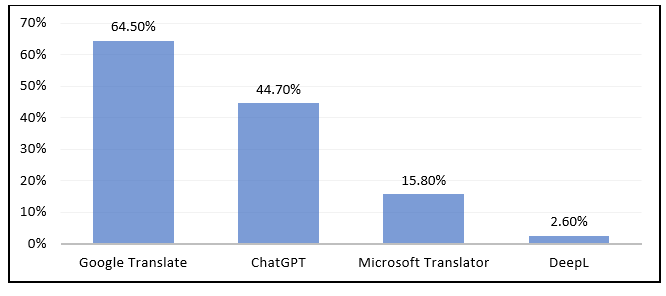
\includegraphics[width=\textwidth]{Figure 3.png}
 \caption{Usage Rates of Translation Tools among Translators.}
 \label{fig3}
 \source{The authors.}
\end{minipage}
\end{figure}

\item \textbf{Frequency of Usage}

\Cref{fig4} illustrates that the vast majority of translators use these tools occasionally in their translation work. This pattern demonstrates that AI-powered tools are integrated into the modern translator’s workflow as a standard aid.

\begin{figure}[htbp]
\centering
\begin{minipage}{.8\textwidth}
 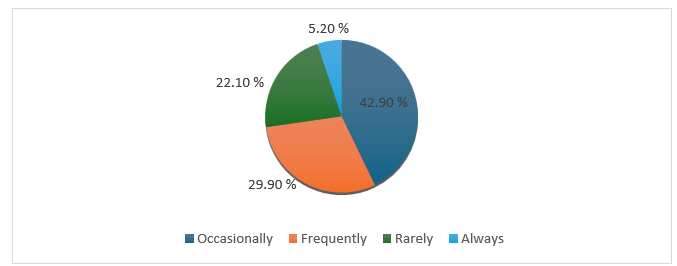
\includegraphics[width=\textwidth]{Figure 4.png}
 \caption{Frequency of Usage of AI-Powered Translation Tools.}
 \label{fig4}
 \source{The authors.}
\end{minipage}
\end{figure}

\item \textbf{Text Types}

The findings revealed a clear and distinct preference, with technical texts being the most frequently cited category at 49.40\%, representing nearly half of all responses. In contrast, the remaining text categories (legal, medical, and media texts) show relatively similar selection rates, clustering within the low- to mid-30 percent range.

\item \textbf{Degree of Satisfaction}

Regarding the translator’s satisfaction degree with the accuracy of AI-powered translation tools, the results showed a positive response, with a combined 46.80\% of participants reporting being “Satisfied” or “Very Satisfied,” as shown in \Cref{fig5}. However, a considerable proportion (40.50\%) of respondents expressed a neutral stance.

\begin{figure}[htbp]
\centering
\begin{minipage}{.8\textwidth}
 
\includegraphics[width=\textwidth]{Fig5.png}
 \caption{Translators’ Degree of Satisfaction with the Accuracy of AI-Powered Translation.}
 \label{fig5}
 \source{The authors.}
\end{minipage}
\end{figure}

\item \textbf{Training on AI-Powered Translation}

Regarding the training on the usage of AI translation tools, the respondents (86.10\%) reported that they have not received any training or formal guidance on how to employ these tools in the translation process, as indicated in \Cref{fig6}. The results also revealed that 71.40\% of participants were self-taught in using such tools.

\begin{figure}[htbp]
\centering
\begin{minipage}{.8\textwidth}
 
\includegraphics[width=\textwidth]{Fig6.png}
 \caption{Training or Guidance on Using AI-Powered Translation Tools.}
 \label{fig6}
 \source{The authors.}
\end{minipage}
\end{figure}

\item \textbf{Advantages of AI-Powered Machine Translation}

Participants identified key advantages of using AI-powered machine translation tools. The majority (79.70\%) highlighted improving translation speed as the most prominent benefit. This emphasizes AI’s ability to offer quick results and enhance workflow efficiency. It was followed by increased translators' productivity (51.90\%) and handling large volumes of texts (41.80\%). A smaller proportion of respondents mentioned increasing consistency in translation (27.80\%) and enhancing translation accuracy (25.30\%). This suggests that while AI translation tools are recognized for operational efficiency, their linguistic precision is viewed with moderate confidence. Overall, these findings indicate that translators primarily value AI technologies for their speed and productivity benefits rather than for improvements in linguistic or contextual quality.

\item \textbf{Disadvantages of AI-Powered Machine Translation}

Regarding the disadvantages of using AI-powered machine translation tools, the results showed that the majority (70.90\%) identified inaccuracies in cultural translation as the most significant drawback, indicating persistent challenges in capturing culture-specific meanings. This was followed by a lack of contextual understanding (65.80\%) and difficulty handling creative or idiomatic expressions (55.70\%), both of which underscore the limitations of AI systems in interpreting implied meanings and non-literal language. Meanwhile, replacing human translators was perceived as a concern by 41.80\% of respondents, reflecting moderate apprehension about job displacement. Finally, ethical concerns were mentioned by 35.40\% of the respondents. Overall, the results emphasize that participants perceive AI translation tools as insufficiently equipped to address complex linguistic and cultural dimensions of translation.

These findings reveal more than just usage statistics. They shed light on how AI tools are integrated into the work of Palestinian translators and their implications for Arabic translation. While adoption is widespread, translators rely on AI mainly for technical and structured texts, reflecting cautious trust in its ability to handle culturally and rhetorically complex material. The findings point to a fundamental tension: while AI streamlines translation processes and enhances output speed, it remains limited in capturing the structural complexity, idiomatic subtleties, and cultural specificity inherent in Arabic texts. This interpretation stresses the novelty of the study, showing that AI serves as a supportive tool rather than a replacement for human judgment in the digital translation of Arabic. Additionally, these findings provide empirical evidence of how AI-powered translation tools are currently integrated into the professional practices of Palestinian translators.
\end{enumerate}


\subsection{RQ 2: How do professional translators perceive the use of AI-powered translation tools in their work, particularly regarding potential advantages and challenges, cultural meaning, and ethical considerations?}\label{sec-links}
This subsection addresses the second research question through the analysis of data collected from the second research instrument, namely, the interviews. The results of this question have been organized thematically, highlighting the key patterns and recurring perspectives shared by professional translators regarding the use of AI-powered translation tools in their translation work. To enhance analytical depth, all reported quotations are accompanied by participants’ experience level and employment profile, enabling comparison between junior and more experienced translators.

\begin{enumerate}
    \item \textbf{Advantages of AI-Powered Machine Translation Tools}

    Participants highlighted several advantages of AI-powered translation tools. These tools were perceived as time-saving and efficient, especially for long texts. They also offered alternative terminology and helped improve cohesion and word choice. As one senior professional with an advanced certificate in translation, working as a freelance translator, noted: “The tools save time and efforts. They are updated regularly, offering more choices.” Another participant, working as a licensed, freelance translator and translation trainer, emphasized their practical utility in specialized fields: “In medical translation, it provided me with a more contextualized terminology.” Additionally, AI tools were valued by the respondents for facilitating legal and technical translations. For them, the tools provided appropriate vocabulary and support for structured translation workflows.

    \item \textbf{Trust in AI-Generated Translations}

    Despite these benefits, trust in AI-generated translations was consistently reported as limited, with human revision seen as essential. Trust was higher for technical or legal texts but considerably lower for literary texts. As one junior translator pursuing her graduate studies and working as a freelancer explained, “for legal texts, 90\% I can rely on it, but for literary texts, I make many adjustments.” Importantly, participants emphasized that AI translations could be misleading without human oversight. One senior translator, working as a freelance academic translator, stated that “there should be human intervention when using these tools.”

    \item \textbf{Challenges with AI Tools}

    Participants identified several challenges when using AI tools, including literal translations, omissions in long texts, and inaccuracies in terminology. One senior translator working in the field of academic translation on a part-time basis observed: “The quality of the translation for longer texts is poor. In academic texts, in-text citations are often deleted.” Another junior translator working as a freelancer added that “it sometimes doesn’t translate all the text. For poetry and literature, it translates literally.” Such challenges highlighted the need for careful human intervention to ensure accuracy and fidelity. Indeed, they highlight AI’s inability to navigate Arabic’s rhetorical complexity, demonstrating that efficiency gains do not equate to contextual or stylistic adequacy.

    \item \textbf{AI’s Role in Maintaining Cultural Meaning and Context}

    A major concern among translators was the ability of AI to preserve cultural meaning and context. Most of them agreed that AI-powered tools struggle with culture-specific phrases and meanings, and further stated that the translation output requires human expertise for accurate rendering. As one junior translator who is pursuing graduate studies in translation explained, “cultural meaning is not included in the resources […]. It is not easy to render culture-specific terms.” Another senior translator with legal translation research interests noted that “some legal phrases are Islam-driven terms […]. If the concept is absent in one culture, that gap cannot be easily rendered by AI.” Translators emphasized that AI translations often reflect general or widely available knowledge but fail to capture culturally embedded meanings, which makes human intervention crucial. This confirms that AI tools currently act as assistive instruments rather than autonomous agents capable of understanding Arabic cultural and rhetorical dimensions.

    \item \textbf{Ethical Considerations in Using AI Tools}

    Ethical considerations were also highlighted. The translators consistently stressed transparency when using AI, particularly in client-facing work, and the importance of reviewing sensitive texts. “It is not ethical to use ChatGPT without informing the clients,” one junior translator working as a freelancer stated, while another senior translator with experience in legal translation added that “personal data are maintained; no names are mentioned in legal documents. I do revisions and corrections where needed.” Overall, participants suggested that AI tools should be used responsibly, primarily to support translators rather than replace human judgment. This positions AI as a complementary tool rather than a replacement, showcasing the study’s contribution to understanding AI adoption in Arabic translation in the digital era.

    Overall, while AI-powered translation tools offer key advantages in terms of efficiency, terminology suggestions, and support for technical texts, professional translators emphasize the necessity of human oversight. Trust remains limited, particularly for literary and culturally embedded texts, and challenges such as literal translations and omissions persist. Ethical use and careful attention to cultural meaning are considered essential, positioning AI tools as a valuable complement rather than a replacement for human expertise. The interview findings provide deeper qualitative insights into translators’ perceptions of AI-powered translation tools and their implications for professional practice. While participants acknowledged the efficiency and terminology support offered by these technologies, they emphasized the need for human intervention to address cultural and contextual meaning and ethical considerations. These findings foreground the continuing importance of human expertise in Arabic translation, particularly when dealing with culturally embedded discourse.
\end{enumerate}


\section{Discussion}\label{sec-outras-estr}
The current study has investigated the extent to which Palestinian professional translators employ AI-powered translation tools, their usage patterns, and satisfaction levels, as well as their perceptions regarding the advantages, challenges, cultural implications, and ethical dimensions of using such technological tools. Through a mixed-methods approach that combined a questionnaire distributed among professional translators and structured interviews with experienced translators, the study provided a comprehensive understanding of how AI technologies are reshaping translation practices in the Palestinian context.

The findings revealed a high level of adoption of AI-powered translation tools, with most translators frequently using platforms like Google Translate and ChatGPT. This widespread usage highlights how AI technologies are increasingly integrated into professional translation workflows due to their speed and efficiency. However, the results reveal a model of selective and strategic reliance, where translators employ AI primarily as an efficient instrument while retaining human oversight for linguistically and culturally complex tasks. Such results are consistent with findings from earlier scholarship stressing the pragmatic yet cautious approach adopted by translators toward AI-assisted translation. \textcite{SahariAlKadiAli2023ChatGPTTranslation} found that translation teachers were satisfied with AI-assisted translation represented in ChatGPT. Similar to the participants of this study, their analysis found that the participants recognized both positive and negative aspects of using ChatGPT in the translation process. Regarding the types of tools used by the Palestinian translators, the present study revealed that translators tend to use Google Translate more frequently than LLM-based tools such as ChatGPT. This preference may stem from Google Translate’s familiarity, accessibility, and integration into translators’ daily workflows, which makes it a more convenient option for quick translation tasks. Another reason might be that ChatGPT is often viewed as a broader conversational tool rather than a specialized translation platform, and many translators may still have limited trust in its accuracy when handling professional translation tasks.

The results also demonstrated that participants of this study expressed confidence in using AI for technical texts. This might be because such texts generally have standardized terminology, clear structures, and limited figurative language. AI systems are usually trained on such consistency in glossaries and structures. \textcite{AlyamiAlzubi2025HumanTranslatorsAI} found that AI has improved efficiency in translation work, particularly in technical translations, where the AI tools maintain consistency through the translation process. Critically, this confidence highlights a distinction between procedural accuracy and rhetorical adequacy. While AI performs effectively in structured and terminology-based genres, it remains less capable of navigating stylistic and implied meaning, as well as culturally embedded discourse.

On the other hand, translators showed a cautious dependence on the AI-powered tools. While translators acknowledge the efficiency and productivity improvements that AI provides, their trust in the accuracy and contextual appropriateness of AI machine translations remains limited, particularly when dealing with culturally embedded references. It could be argued that AI systems often struggle with culture-specific references because the related expressions are deeply rooted in social, historical, and linguistic contexts that go beyond the literal meaning. In addition, they may not have direct equivalents in the target language and require further interpretation and adaptation that only human translators can provide. This limitation is particularly significant in Arabic, a language characterized by rich morphology and culturally dense expressions that demand interpretive judgment rather than literal transfer. Such concerns related to the culture-specific terms and meanings are also reflected in the literature. \textcite{Shahmerdanova2025AITranslation} argues that AI machine translations still struggle with idiomatic expressions and culturally specific idioms. She advocates for integrating AI technology with human experience to address such issues and thus enhance global communications. In this vein, \textcite{AlMaaytah2026EvaluatingNMT} states that cultural misinterpretations are expected in idiomatic and context-dependent translations in machine translation. Similarly, \textcite{CorpasPastorNoriegaSantianez2024Creativity} note that the adoption of NMT technology in translation has not fully extended to the creative domain of literary translation, a field that is inherently rich in culture-specific references and culturally bound expressions. Arguably, AI systems continue to struggle to render such elements accurately. Thus, the findings position human translators not merely as post-editors but as cultural mediators responsible for preserving rhetorical integrity and contextual authenticity.


\section{Conclusion}\label{sec-listas}
The current study has addressed two research questions by providing evidence of how translators adopt and use AI tools (RQ1) and how they perceive their advantages, limitations, and ethical implications (RQ2), thereby contributing novel insights into human-AI collaboration in Arabic translation practice. These findings have significant implications for translation pedagogy, professional development, and industry practice.

First, translation training programs in academic and professional settings should incorporate AI literacy while fostering critical awareness of linguistic and cultural limitations. Structured training on AI-powered translation tools would help translators leverage technology responsibly while maintaining quality standards and ethical integrity. Importantly, such training should also equip translators to evaluate, adapt, and ethically supervise machine-generated output rather than passively accept it. Second, professional translation associations and local institutions should facilitate workshops and continuous professional development initiatives to bridge the gap between technology adoption and professional proficiency. Third, AI developers and translation researchers should collaborate to improve the contextual and cultural sensitivity of AI systems, ensuring that future tools better account for linguistic diversity and cultural nuance. At the same time, translators should remain attentive to the ideological and cultural dimensions of texts throughout the translation process, a principle that continues to be essential even when technology is involved \cite{BadahEtAl2026Recontextualization}.

Overall, this study contributes to the growing body of literature on human-AI collaboration in translation, reinforcing the position that while AI offers undeniable advantages in speed and efficiency, human expertise remains indispensable for ensuring cultural accuracy and ethical responsibility, particularly in post-editing AI-generated drafts to resolve ambiguities, cultural nuances, and figurative language \cite{ShehabBadah2026ConversationalImplicatures}. By explicitly linking the conclusions to both research questions, the study clarifies how AI adoption and usage (RQ1) intersect with professional perceptions of advantages, limitations, and ethical use (RQ2). By foregrounding the specific challenges associated with Arabic in the digital age, the study advances a critical understanding of AI not as a replacement for human translators but as a technology that reshapes professional roles and responsibilities. Future research could extend the current investigation in several directions. Longitudinal studies would be valuable in tracking how translators’ attitudes evolve as AI technologies continue to advance.


\printbibliography\label{sec-bib}
% if the text is not in Portuguese, it might be necessary to use the code below instead to print the correct ABNT abbreviations [s.n.], [s.l.]
%\begin{portuguese}
%\printbibliography[title={Bibliography}]
%\end{portuguese}


%full list: conceptualization,datacuration,formalanalysis,funding,investigation,methodology,projadm,resources,software,supervision,validation,visualization,writing,review
\begin{contributors}[sec-contributors]
\authorcontribution{Amjad Mohammad Badah}[conceptualization,datacuration,formalanalysis,investigation,methodology,resources,validation,visualization,writing,review]
\authorcontribution{Laura Esteban-Segura}[methodology,validation,supervision,review]
\end{contributors}

\section*{\fontsize{10}{12}\selectfont AI statement}
The researchers used AI-assisted tools solely to improve the readability of this article and retain full responsibility for the accuracy and integrity of its content.

\begin{dataavailability}
\txtdataavailability{dataonly} % options: dataavailable, dataonly, databody, datanotav, nodata
\end{dataavailability}


\appendix 

\section*{Appendix A -- Study Questionnaire}

\subsection*{Translation in the Age of AI: Insights from Palestinian Professional Translators}

Dear Professional Translator,

Recently, the landscape of translation has witnessed important advancements with the introduction of Artificial Intelligence (AI) in the translation industry. As we experience this dynamic landscape, your perspectives and insights as a professional translator are of high importance in contributing to a better understanding of the integration of AI-powered translation tools in the field of translation.

Please take a few moments to complete the survey thoroughly. Your input is invaluable, and we appreciate your time and effort in contributing to this study. All information provided will be treated with confidentiality, and the results will be presented in an aggregated and anonymized form. Your participation is voluntary, and you may withdraw at any point.

Thanks in advance.

\bigskip

\subsection*{Section One: Demographic Information}

\begin{itemize}

\item \textbf{Gender}
\begin{itemize}
    \item Male.
    \item Female.
\end{itemize}

\item \textbf{Education Background}
\begin{itemize}
    \item Bachelor's Degree (Translation, English Language, English Language Education).
    \item Master's Degree (Translation, Linguistics, Methods of Teaching English).
    \item PhD (Translation or a related field).
    \item Other (please specify).
\end{itemize}

\item \textbf{Translation Experience}
\begin{itemize}
    \item 1--5 years.
    \item 6--10 years.
    \item 11--15 years.
    \item 16+ years.
\end{itemize}

\item \textbf{Employment Type}
\begin{itemize}
    \item Full-time translator (employed by a company or an organization).
    \item Part-time translator.
    \item Freelance translator.
\end{itemize}

\end{itemize}

\subsection*{Section Two: Usage of Artificial Intelligence-Based Machine Translation}

\begin{itemize}

\item \textbf{Do you use AI-powered machine translation in translation? If no, you can click ``Next,'' then submit the form.}
\begin{itemize}
    \item Yes.
    \item No.
\end{itemize}

\item \textbf{If yes, please specify the AI-powered translation tools that you use:}
\begin{itemize}
    \item Google Translate.
    \item ChatGPT.
    \item Microsoft Translator.
    \item DeepL.
    \item Other (please specify).
\end{itemize}

\item \textbf{How frequently do you use AI-powered translation tools?}
\begin{itemize}
    \item Rarely.
    \item Occasionally.
    \item Frequently.
    \item Always.
\end{itemize}

\item \textbf{What type of texts do you usually translate using AI-powered machines? Please select all that apply.}
\begin{itemize}
    \item Technical Texts.
    \item Legal Texts.
    \item Medical Texts.
    \item Media Texts.
    \item Other (Specify).
\end{itemize}

\item \textbf{How satisfied are you with the accuracy of AI-powered translation tools?}
\begin{itemize}
    \item Very Satisfied.
    \item Satisfied.
    \item Neutral.
    \item Dissatisfied.
    \item Very Dissatisfied.
\end{itemize}

\item \textbf{Have you received any training or guidance on using AI-powered translation tools?}
\begin{itemize}
    \item Yes.
    \item No.
\end{itemize}

\item \textbf{If yes, please indicate the source of your training. Select all that apply.}
\begin{itemize}
    \item Training provided by your employer.
    \item Self-learned.
    \item Formal education (e.g., courses, workshops).
    \item Other (please specify).
\end{itemize}

\item \textbf{In your opinion, what are the main advantages of using an AI-powered machine in translation? Please select all that apply.}
\begin{itemize}
    \item Improving translation speed.
    \item Enhancing translation accuracy.
    \item Increasing consistency in translation.
    \item Handling large volumes of texts efficiently.
    \item Increasing translator's productivity.
    \item Other (please specify).
\end{itemize}

\item \textbf{In your opinion, what are the main disadvantages of using an AI-powered machine in translation? Please select all that apply.}
\begin{itemize}
    \item Encountering ethical concerns.
    \item Facing inaccuracies in cultural contexts.
    \item Handling creative or idiomatic expressions inefficiently.
    \item Lacking contextual understanding.
    \item Replacing human translators.
    \item Other (please specify).
\end{itemize}

\end{itemize}

\section*{Appendix B -- Interview Questions}

\begin{enumerate}

\item Based on your experience, what are the main advantages of using AI-powered machine translation?

\item Can you share specific examples where the use of AI tools has significantly facilitated the translation process?

\item To what extent do you trust AI-generated translations, and how does this influence your final edits and revisions?

\item Have you had to make any significant adjustments to your work processes when adopting these tools?

\item Have you encountered any specific challenges when incorporating AI tools into your translation process?

\item What are your opinions regarding the application of AI in translation, especially concerning its ability to maintain cultural meaning and context?

\item How do you address ethical considerations when you decide to use AI-enhanced translation tools for a certain translation task?

\end{enumerate}

\end{document}

